\documentclass{article}
\usepackage{graphicx} % Required for inserting images
\usepackage{biblatex} % Required for bibliography
\usepackage{hyperref} % Required for references

\addbibresource{ref.bib}

\title{Mini-project - DD2417 - NLP \\ Question word prediction}
\author{
    Tristan Perrot \\ \href{mailto:tristanp@kth.se}{tristanp@kth.se}
    \and Romain Darous \\ \href{mailto:darous@kth.se}{darous@kth.se}
}
\date{March 2024}


\begin{document}

\maketitle
\begin{center}
    
\includegraphics[width = 40mm]{images/KTH_logo_RGB_svart.png}
\end{center}

\begin{abstract}
    This report presents the results of the mini-project for the course DD2417 - Natural Language Processing at KTH. The goal of the project is to predict the question word of a question given the rest of the question and the answer. We present the dataset, different models and the results of the project. We also discuss the limitations of the model and the possible improvements that could be made.
\end{abstract}

\section{Relevant Background}

Natural Language Processing (NLP) encompasses a variety of tasks including text generation, error recovery, translation, and more. Despite their diverse objectives, these tasks share a common aim: given a sequence of strings, the ability to predict the subsequent text or deduce missing elements based on contextual information.

Generative AI tools like ChatGPT or Gemini have showcased the remarkable capabilities of text generation models. Their performance is so impressive that it might seem plausible to address our problem by simply inputting the partial question and obtaining complete it through a Large Language Model (LLM). However, these models are trained on extensive datasets and complex architectures. As our project focus on a specific NLP task, it's worth exploring whether we can construct a more straightforward model, trainable on a smaller dataset and within a reasonable timeframe.

One initial idea is to employ a Multilayer Perceptron (MLP) \cite{popescu2009multilayer} network with a context window to aggregate the embedding of several dictionary elements. However, this approach demands a fixed input size and struggles with retaining long-term memory.

To accommodate inputs of varying lengths, recurrent neural networks (RNNs) have demonstrated superior performance. Models utilizing Long Short-Term Memory (LSTM) units, for instance \cite{santhanam2020context}, have exhibited promising results. A significant breakthrough came with Transformers and the introduction of attention mechanisms \cite{vaswani2017attention}. While traditional text generation models relied on recurrent neural networks, this novel architecture dispenses with such complexities and delivers remarkable outcomes. By stacking Transformers and employing bidirectional attention, models like BERT \cite{devlin2019bert} have been developed and show stunning results regarding information recovery in gap-fill texts.

Each model begins with the construction of a vocabulary, which can be word-based, phoneme-based, or character-based. A spectrum of methods exists, ranging from elementary to cutting-edge approaches. An essential consideration lies in vocabulary embedding. From traditional indexing to more advanced techniques such as Word2Vec \cite{mikolov2013efficient}, a multitude of approaches exist. For the sake of simplicity, our embedding will remain simple here and we won't use any pre-trained Deep Learning model.

This project will explore three distinct methodologies: implementing a classifier for question recovery using LSTM units, constructing a Transformer-based character-by-character prediction model, and comparing these approaches against the pre-trained BERT model.

\section{Dataset}

For the data, we needed a huge Question - Answer dataset. That is why we used the SQuAD2.0 dataset \cite{squad}. This dataset comprises a substantial collection of questions and answers, specifically designed to train models in distinguishing between answerable and unanswerable questions using contextual information. Consequently, we have selected only the questions that had corresponding answers and did not utilize the surrounding context of the questions. Thus, the sole context available for the model to learn from is the content of the questions themselves and the answer associated.

\section{Models}

\subsection{Classifier}

\subsubsection{Motivation}

As said upper, we wanted firstly to answer the question word prediction problem as a classification problem. That's why, we listed possible question words (that could be more than a single word like 'In what' or 'In which'). Therefore, we merged each question and answer without the question word and classify it. We use \textbf{70292} questions / answers and hold 20\% of them for validation and tests.

\subsubsection{LSTM}

For the first classifier, we used an Long Short-Term Memory (LSTM) word based model \cite{lstm1997}. After merging the question and answer, and inverting the sequence to place the prediction at the end, we trained a single-layer LSTM network with an embedding layer. The primary objective of employing the LSTM architecture was to leverage its capabilities for NLP tasks, thereby enabling the classification of the input among all possible question words.

\subsubsection{BERT}

We aimed to implement a BERT classification model. BERT \cite{devlin2019bert}, which stands for Bidirectional Encoder Representations from Transformers, is a language model rooted in the transformer architecture \cite{vaswani2017attention}. It is designed for word prediction, leveraging training that involves masking and unmasking words within texts. We utilized a pre-trained BERT model and fine-tuned it for our specific task. Similar to the LSTM model, this model operates on words rather than characters. For our task, we masked each question word and combined each question with its corresponding answer as before, omitting the flipping process due to the attention-based nature of the model.

\subsection{Character per character question prediction}

\subsubsection{Motivation}
The task of completing a question typically involves recovering only a few words, here no more than two. Despite this small number, considering the size of the vocabulary is crucial. Questions can vary greatly in their formulation, whether spoken or written, including the use of prepositions, choice of auxiliary, and other linguistic nuances. This diversity makes it challenging to train a model to predict the most likely word, especially given the extensive vocabulary compared to the dataset size.

However, the character count needed remains consistent, limiting the potential outputs to a manageable level. Additionally, the characters required for completion are often similar across different questions. This scenario makes a character prediction model quite relevant, as it may not excel at predicting long strings but could effectively recover one or two words.

\subsubsection{The vocabulary and dataset adaptation}
Here the vocabulary will be the characters present in the dataset. We will not use any embedding method, but only sequential indexing of the characters, to keep the model simple. 

\subsubsection{Dataset and labels}
Each data point in our dataset consists of a question and its answer concatenated together. We chose to include unanswerable questions as well, as their formulation often resembles answerable ones, especially at the beginning, which is our focus for recovery.

Since the words we aim to recover are always at the start of the question, we decided to reverse their characters. For example, "How are you? I am fine." becomes ".enif ma I? uoy era woH". This transforms our problem into predicting the next character given the preceding context.

For each data point, we begin with all the characters up to those of the last two words in the question as features. The label is the subsequent character. Using a sliding context window, we generate multiple data points from a single sentence by sequentially adding the characters of the two words we aim to recover as features and using the next character as the label. We also introduce a special token, \textbf{"BOQ"} (Beginning Of Question), to indicate where the model should stop when predicting a question.

Here's a step-by-step example of dataset construction:

\begin{itemize}
    \item \textbf{Raw Data Point:} "How are you? I am fine."
    \item \textbf{Reversed Raw Data Point:} ".enif ma I? uoy era woH"
    \item \textbf{Features:} ".enif ma I? uoy "
    \item \textbf{Label:} "e"
    \item Replace characters with their index,
    \item Shift the context window to the right,
    \item \textbf{Features:} "enif ma I? uoy e"
    \item \textbf{Label:} "r"
    \item Replace characters with their index,
    \item Repeat for subsequent characters.
\end{itemize}


\subsubsection{The model}
We decided to use \textbf{tacked transformers} to perform character-per-character prediction with multi-head attention. Hyperparameters will be given in section \ref{cpc_hyperparams}.
We decided to use \textbf{causal attention} only given the past context.

\subsubsection{Computing the context}

Regarding how to compute the \textbf{context}, we tried two different approaches. 

\begin{itemize}
    \item \textbf{Sequential context}: The usual context where features consist of the previous characters within a window length.
    \item \textbf{Split context}: We compel the model to consider the answer if the question is too long. We believe the answer could provide valuable insights into completing the beginning of the question.
\end{itemize}

\section{Results}

\subsection{Classifiers}

\subsubsection{LSTM}

For the training process, we used cross entropy loss and Adam optimizer. Figure \ref{fig:lstm-loss} shows the loss of training with early stopping with patience.

We obtain an accuracy on the test set of \textbf{73.26\%} which is quite good for this model. For a better evaluation of the performance, we used confusion matrix on the test dataset to see how well the model was behaving. The figure \ref{fig:lstm-conf} is that matrix. We can see that some words are better predicted than others. For example, the model predicts a lot of time \texttt{What} instead of \texttt{Why}. However, the model predicts really well words like \texttt{Why} and \texttt{What} when they are targeted. We can also see that some words were predicted whereas they never appear in the dataset initially.

\subsubsection{BERT}

Due to the power of the BERT architecture, we achieve to get, on the test set, an accuracy of \textbf{90\%} which is really great.
Like before, we plotted and the confusion matrix in figure \ref{fig:bert-conf}. There, we can see that BERT clearly outperform the LSTM classifier. Almost every question words are well predicted. We can see that there is a small confusion on the words \texttt{What} and \texttt{Which} which is not surprising because they are quite similar and both could be used depending on the context. We can see here the power of self-attention and that we can achieve really great results for classification based on NLP.

\subsection{Character per character question prediction}

\subsubsection{Hyperparameters}\label{cpc_hyperparams}

\begin{itemize}
    \item \textbf{Number of Transformer Encoders:} 2
    \item \textbf{Number of Attention Heads:} 2
    \item \textbf{Hidden Size:} 64
    \item \textbf{Dropout Probability:} 0.1
    \item \textbf{Patience (Early Stopping):} 5
    \item \textbf{Batch Size:} 64
    \item \textbf{Optimizer:} Adam
    \item \textbf{Learning Rate:} 0.0003
    \item \textbf{Weight Decay:} 0.000001
    \item \textbf{Number of Epochs Max:} 100
    \item \textbf{Is Causal:} True (When True, the attention is causal)
    \item \textbf{Sequential Context:} True or False (True : Sequential context ; False Split context)
    \item \textbf{Maximum Length of context:} 32 or 64
\end{itemize}

We will perform a \textbf{grid search} on the context parameters to try to find a suitable choice. It gives a total of 4 models trained.

\subsubsection{Model choice}

Overall, the models were quick to train, converging after a few iterations and stopping based on the patience criteria.

Figure \ref{fig:cpc_eval} shows the results of training the four models. Overall, they have similar performance with a low test accuracy, barely reaching 25\%. By testing our model on examples, we observed that some interrogation words were correctly recovered and that the stopping token \textbf{BOQ} was often well predicted, ensuring that the question recovery stops correctly.

We tried to stacking more encoders or to increase the hidden dimension, but it did not help improve the results; it made the model too complex and led to overfitting.


\section{Conclusion}
In this project, we explored different models for predicting question words given the rest of the question and the answer. The character-by-character models, despite their flexibility, were too simplistic, reaching only 25\% accuracy.

The BERT model performed best, achieving a test accuracy of 90\%, proving the efficiency of pre-training. Conversely, the LSTM model achieved a lower accuracy of 73.26\%. These two models performed well but with a very small vocabulary. Future work could focus on expanding the vocabulary of BERT, our best performing model, to see how it performs with a more realistic range of words.

\medskip

\newpage

\printbibliography

\newpage

\appendix

\section{Classification results}

\subsection{Training}

\begin{figure}[ht]
    \centering
    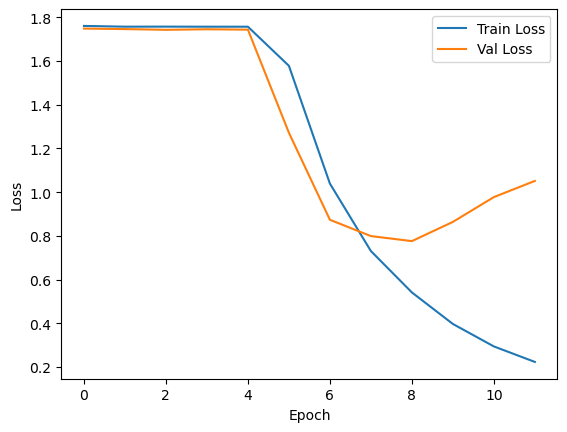
\includegraphics[width=0.8\linewidth]{results/classification/lstm loss.png}
    \caption{LSTM training loss}
    \label{fig:lstm-loss}
\end{figure}
\newpage
\subsection{Confusion matrices}

\begin{figure}[ht]
    \centering
    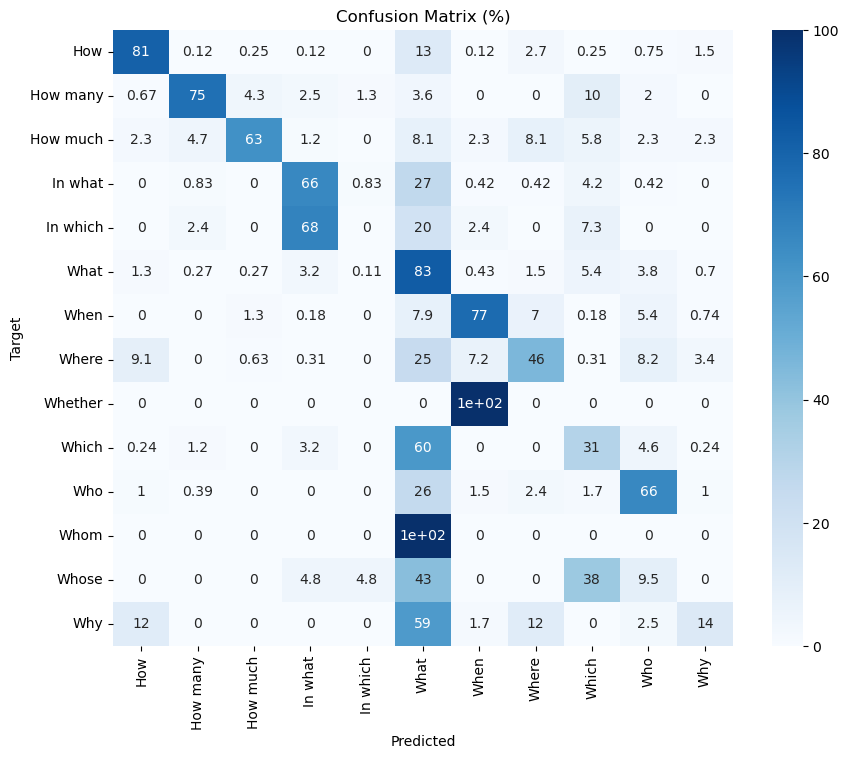
\includegraphics[width=0.75\linewidth]{results/classification/lstm conf.png}
    \caption{LSTM confusion matrix}
    \label{fig:lstm-conf}
\end{figure}

\begin{figure}[ht]
    \centering
    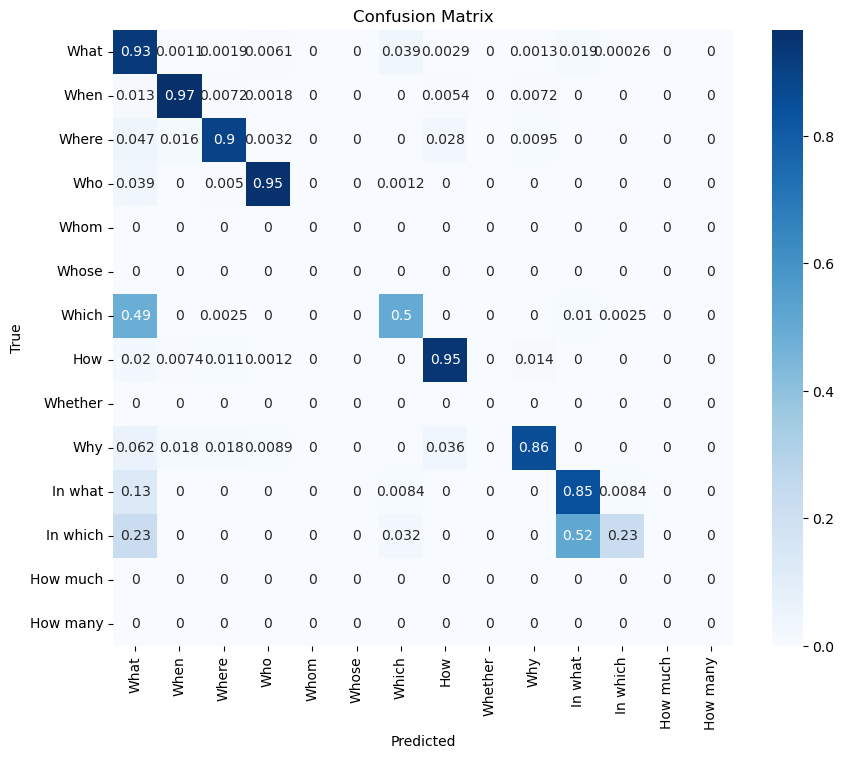
\includegraphics[width=0.75\linewidth]{results/classification/conf bert.png}
    \caption{BERT confusion matrix}
    \label{fig:bert-conf}
\end{figure}
\newpage\newpage
\section{Character per character model}

\begin{figure}[ht]
    \centering
    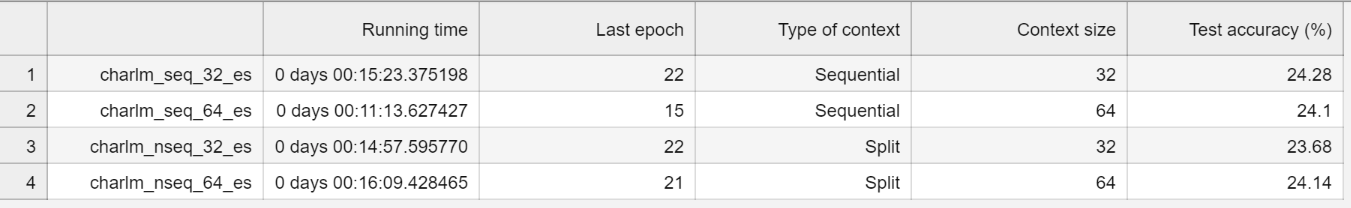
\includegraphics[width=1.2\linewidth]{results/evaluation.png}
    \caption{Evaluation of the four trained models.}
    \label{fig:cpc_eval}
\end{figure}

\end{document}
